\documentclass[13pt]{beamer}				\usepackage{graphicx}
\usepackage{comment}
\usepackage{pdfpages}	
\usepackage{tikz}
\usetikzlibrary{mindmap}
\usepackage{comment}
\usepackage{relsize}
\usepackage{mathtools}
\usepackage{biblatex}
\addbibresource{biblio.bib}

\newcommand\Ccancel[2][black]{\renewcommand\CancelColor{\color{#1}}\xcancel{#2}}
\mode<presentation>						% Set options
{
  \usetheme{Madrid}					% Set theme
  \usecolortheme{seahorse} 				% Set colors
  \usefonttheme{default}  				% Set font theme
  \setbeamertemplate{caption}[numbered]	% Set caption to be numbered
}
\usepackage[makeroom]{cancel}
\definecolor{blue}{RGB}{88, 88, 191}
\definecolor{white}{RGB}{255, 255, 255}
\definecolor{uuuuuu}{rgb}{0.2666,0.2666,0.2666}
\definecolor{wwwwww}{rgb}{0.4,0.4,0.4}
\definecolor{ccqqqq}{rgb}{0.8,0,0}
\definecolor{qqqqff}{rgb}{0,0,1}


\usepackage{hyperref}					% For cross-referencing

\title[Message Passing Graph Neural Networks]{Message Passing Graph Neural Networks}
\author[Polina Barabanshchikova]{Polina Barabanshchikova}	
\institute[MIPT]{MIPT}
\DeclareMathOperator{\rank}{rank}
\DeclareMathOperator{\dist}{dist}
\DeclareMathOperator{\conv}{conv}
\DeclareMathOperator{\tr}{tr}
\DeclareMathOperator{\degree}{deg}
\DeclareMathOperator{\cl}{cl}
\DeclareMathOperator{\argmin}{argmin}
\DeclareMathOperator{\lo}{\longleftrightarrow}
\DeclareMathOperator{\Lo}{\Longleftrightarrow}
\newcommand{\D}{\overline{D}}
\begin{document}

\begin{frame}
  \titlepage
\end{frame}

\begin{frame}{Motivation}
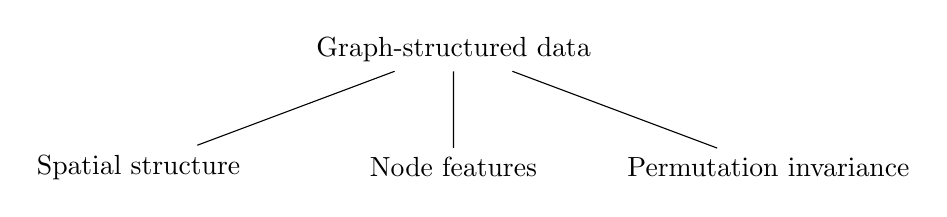
\begin{tikzpicture}[align=flush center, 
level/.style={sibling distance=40mm/#1}]

\node{Graph-structured data}
	child { node {Spatial structure}}
	child { node {Node features}}
	child { node {Permutation invariance}}
;
\end{tikzpicture}
\end{frame}

\begin{frame}{Intuition}
\begin{figure}[h!]
    \includegraphics[width=1\textwidth, trim={0 0 0 0cm},clip]{mpnn1.png}
\end{figure}
\begin{figure}[h!]
    \includegraphics[width=0.5\textwidth, trim={0 0 0 0cm},clip]{mpnn2.png}
\end{figure}
\href{https://towardsdatascience.com/the-intuition-behind-graph-convolutions-and-message-passing-6dcd0ebf0063}{\tiny{\nolinkurl{https://towardsdatascience.com}}}
\end{frame}

\begin{frame}{Problem statement}
Given a graph $G = (V, E)$ with node features $x_v, v\in V$ and edge features $e_{v w}, (v, w) \in E$, there are two types of tasks
\begin{itemize}
\item Predict label or value for graph classification or regression
\item Predict label or value for each node or edge in structured prediction
\end{itemize}
\end{frame}

\begin{frame}{Method description}
\textbf{Message passing neural networks (MPNN)}

Let $h^t_v$ represent the node embedding for some vertex $v$ at iteration t.

\textbf{1. Initialization}
$$h^{(0)}v = x_v \;\;\;\; \forall v \in V$$
\pause

\textbf{2. Message passing phase}
For $1 \leq t < T$
$$m_v^{t+1} = \sum \limits_{w \in N(v)} M_t(h_v^t, h_w^t, e_{vw})$$
$$h_v^{t+1} = U_t(h_v^t, m_v^{t+1})$$
where $N(v)$ denotes the neighbors of $v$ in $G$.
\pause

\textbf{3. Readout phase}
$$\hat{y} = R(\{h_v^T | v \in G\})$$
\end{frame}

\begin{frame}{Message passing function}
\begin{itemize}
\item \textbf{Concatenation}
$$M_t(h_v^t, h_w^t, e_{vw}) = (h_w^t, e_{vw})$$
\item \textbf{Matrix Multiplication}
$$M_t(h_v^t, h_w^t, e_{vw}) = A_{e_{vw}}h_w^t$$ (for discrete edge types)
\item \textbf{Edge Network}
$$M_t(h_v^t, h_w^t, e_{vw}) = A(e_{vw}) h_w^t,$$ where $A(e_{vw})$ is a neural network which maps the edge vector to a $d\times d$ matrix
\item \textbf{Pair Message}
$$M_t(h_v^t, h_w^t, e_{vw}) = f(h_v^t, h_w^t, e_{vw}),$$ where $f$ is a neural network
\end{itemize}
\end{frame}

\begin{frame}{Update function}
\begin{itemize}
\item \textbf{Sum} 
$$U_t(h_v^t, m_v^{t+1}) = h_v^t + m_v^{t+1}$$
\item \textbf{MLP}
$$U_t(h_v^t, m_v^{t+1}) = \sigma(H_t^{deg(v)} m_v^{t+1})$$
\item \textbf{RNN} 
$$U_t(h_v^t, m_v^{t+1}) = GRU(h_v^t, m_v^{t+1})$$
the same update function at each time step $t$
\end{itemize}
\end{frame}

\begin{frame}{Readout function}
\begin{itemize}
\item \textbf{Neural Network}
$$R = f(\sum \limits_{v \in G} h_v^T)$$
$$R = \sum \limits_{v \in G} f(h_v^T)$$
\item \textbf{Neural Network with skip connections}
$$R = f\left(\sum \limits_{v, t} \text{softmax}(W_t h_v^t)\right)$$
\item \textbf{Two Neural Networks}
$$R = \sum \limits_{v \in G} \sigma \left(f_1(h_v^T, h_v^0)\right) \odot \left(f_2(h_v^T)\right),$$
where $\odot$ denotes elementwise multiplication
\end{itemize}
\end{frame}

\begin{frame}{Virtual graph elements}
Allow information to travel long distances during the propagation phase
\begin{itemize}
\item \textbf{Virtual edge} for pairs of nodes that are not connected
\item \textbf{Master node} which is connected to every input node in the graph with a special edge type. Master is allowed to have a separate node dimension
\end{itemize}
\end{frame}

\begin{frame}{Application}
\textbf{Molecular property prediction}

Experiments
\begin{itemize}
\item Any $T \geq 3$ works
\item Complete edge feature vector (bond type, spatial distance) and explicit hydrogen work better
\item Common weights and a large hidden dimension are beneficial
\item The pair message function performs worse than the edge network function 
\end{itemize}

\end{frame}

\begin{frame}{Literature}
\nocite{mpnn}
\printbibliography
\end{frame}

\begin{frame}{Questions}
\textbf{1.} What function do virtual elements perform?

\textbf{2.} Describe the three stages of MPNN

\end{frame}

\end{document}